\begin{figure}[h!]
	\centering
	\begin{minipage}[b]{1\textwidth}
    		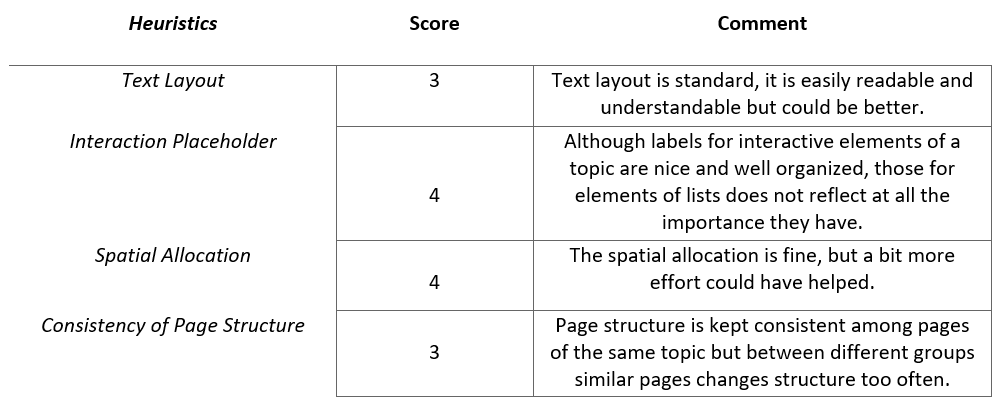
\includegraphics[width=\textwidth]{./assets/layout-final.PNG}
	\end{minipage}
\end{figure}
\FloatBarrier

\subsubsection{Text Layout}
Text layout is easily readable, but sometimes the font size is too small (10.5) and, with a longer text, it results more difficult to read it. Events and accomodations' cards could look tidier by adjusting image and text heights, by reducing titles dimension, justifing text, without truncating it in the middle of a word and by giving it a bottom margin. Some cards, such as figure 6.a, respect the charateristics described above but most of them are shaped as figure 7.

\begin{figure}[h!]
	\centering
	\begin{minipage}[b]{1\textwidth}
    		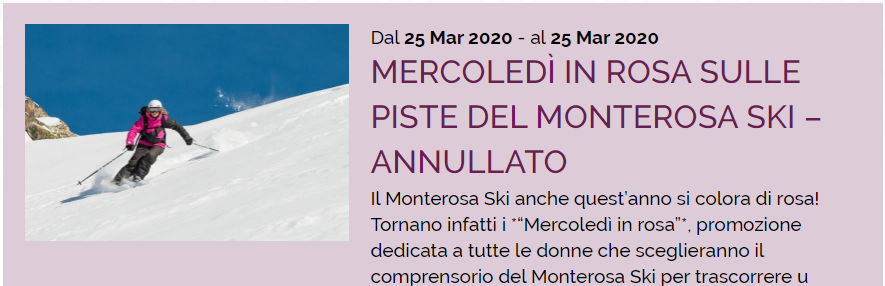
\includegraphics[width=\textwidth]{./assets/event.png}
		\caption{Untidy event card}
	\end{minipage}
\end{figure}
\FloatBarrier

\subsubsection{Interaction Placeholder}
Textual and visual labels are expressive almost in every case, a small flaw is given by some textual links that aren't underlined and that, for this reason, seem to be normal and not clickable text. There are some inconcistency, such as the fact that all topbar elements are linked to general pages except for the textual label "Vacanze su misura" or the way in which filter buttons are labeled and shown. Some navigation buttons are expressive and consistent but could have a different layout (they could be bigger) in order to be more effective.

\subsubsection{Spatial Allocation}
Text and contents are well placed and reflect their relevance, but these elements could use pages' horizontal space in a better way.

\subsubsection{Concistency of Page Structure}
Pages belonging to the same groups or topics have similar layouts and they are consistent, but pages of different groups that are supposed to have same function aren't consistent and often have a different structure.